\documentclass[border=3mm]{standalone}

\usepackage{xcolor}

\usepackage{tikz}
\usetikzlibrary{shapes,decorations,shadows}

\usetikzlibrary{calc}


\usetikzlibrary{decorations.text}



\begin{document}


\tikzset{paint/.style={ draw=#1!50!black, fill=#1!50 },
    decorate with/.style=
    {decorate,decoration={shape backgrounds,shape=#1,shape size=2mm}}}




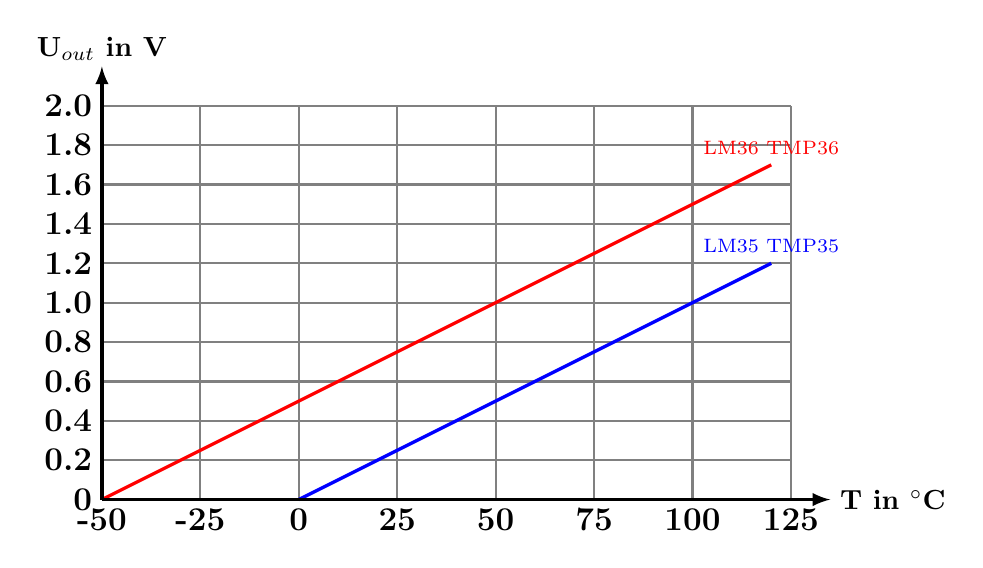
\begin{tikzpicture}
  % grid 
  \draw[help lines,thick, xstep=1.25,ystep=.5] (-2.5,0) grid (6.25,5);
  \foreach \x in {-50,-25,...,125} { \node [anchor=north] at (\x/20,0) {\bf \large\x}; }
  \foreach \y in {0,0.2,0.4,0.6,0.8,1.0,1.2,1.4,1.6,1.8,2.0} { \node [anchor=east] at (-2.5,\y*2.5) {\bf \large\y}; }
  \draw[very thick,color=red] (-2.5,0) -- (6,4.25) node[above,font=\scriptsize] {LM36 TMP36};
  \draw[very thick,color=blue] (0,0) -- (6,3.) node[above,font=\scriptsize] {LM35 TMP35};
  %axis
  \draw[-latex,very thick] (-2.5,0) -- coordinate (x axis mid) (6.75,0);
  \draw[-latex,very thick] (-2.5,0) -- coordinate (y axis mid) (-2.5,5.5); 
  \node [anchor=north] at (-2.5,6) {\bf U$_{out}$ in V};
  \node [anchor=west] at (6.75,0) {\bf T in $\null^\circ$C};
\end{tikzpicture}


\end{document}